\documentclass[twocolumn,10pt,a4paper]{article}
\usepackage[margin=0.75in]{geometry}
\usepackage[utf8]{inputenc}
\usepackage[T1]{fontenc}
\usepackage{lmodern}
\usepackage{microtype}
\usepackage{cite}
\usepackage{url}
\usepackage{hyperref}
\usepackage{xcolor}
\usepackage{enumitem}
\usepackage{tabularx}
\usepackage{booktabs}
\usepackage{graphicx}
\usepackage{tikz}
\usetikzlibrary{positioning,arrows.meta,fit,calc}
\hypersetup{colorlinks=true,citecolor=blue,linkcolor=blue,urlcolor=blue}

\title{Paper 0: Human-Governed Intelligence Augmentation for Closed-Loop O-RAN Cloud RAN Day-2 Operations}

\author{David Kypuros \\
\small Red Hat \\
\small \texttt{dkypuros@redhat.com}}

\date{31 May 2026}

\begin{document}
\maketitle

\begin{abstract}
Paper 0 in this five-paper series frames the work as human-governed intelligence augmentation. Closed-loop automation for Cloud RAN is often described as an autonomous agent problem: telemetry enters, an AI system reasons, and a remediation action exits. That framing is unsafe and incomplete for O-RAN Day-2 operations because the operating environment is cyber-physical, standards-governed, and shared across multiple organizational authorities. This paper introduces the top-level frame used by the O-RAN Agent Harness: human-governed intelligence augmentation. The harness is positioned between a managed O-RAN/O-Cloud environment and a human operations authority. Its shared remediation spine is observation, RCA, \texttt{RemediationProposal}, schema validation, sandbox and five-subcheck policy guardrail review, human challenge and co-authorization, TMF688-shaped audit, O2 IMS/TMF921 standards-shaped dispatch, and native reconciler execution. The contribution of this overview paper is not a new interface or a live production interop claim. It is a control architecture vocabulary that explains why the architecture, standards-bridge, research-harness, and structural-communication papers form one cohesive five-paper series.
\end{abstract}

\section{Introduction}

Cloud RAN Day-2 operations sit at an unusual boundary. A fault may begin as a physical timing drift on an Intel E810 NIC, surface as a linuxptp state transition, propagate through Kubernetes and O-RAN Cloud Notifications, require a reasoning step across platform, RAN, and hardware facts, and end as either a service-layer coordination request or an infrastructure-layer change to a host configuration, driver, or firmware contract. The operational problem is not simply classification. It is the safe conversion of multi-vendor evidence into a bounded proposal that a human can understand, edit, approve, or freeze.

A prior multivendor diagnostic publication established a substrate for Cloud RAN troubleshooting \cite{multivendor_blog_2026}. The companion closed-loop work asks what must be added after diagnosis: a route from root cause to action, a proposal shape that can be validated, a standards-shaped delivery surface, an audit envelope, a reversibility profile, and a human authorization point. Four companion papers answer those details: the architecture paper describes the O2-IMS-to-operator-CRD bridge, the standards paper describes the cross-body bridge map, the research-harness paper describes the fixture-driven verification method, and the structural-communication paper explains how schema-bounded artifacts contain AI nondeterminism at the execution boundary. This paper supplies the missing overview: the harness is an intelligence-augmentation system inside a human-governed O-RAN operating environment.

The term \textbf{intelligence augmentation} is used deliberately. The harness does not replace the network operator. It compresses the time from signal to evidence, from evidence to root cause, from root cause to candidate remediation, and from remediation to rollback-aware audit. The final authority to change physical infrastructure remains human. The desired outcome is not autonomous control; it is a better human decision at the dangerous point where software intent becomes a physical or service-affecting change.

\section{The Managed O-RAN Operating Environment}
\label{sec:environment}

We use \textbf{managed O-RAN operating environment} for the full system in which the harness acts. It includes four layers.

\textbf{Standards control environment.} O-RAN WG1 and WG6 define the O-RAN architecture, O-Cloud resource model, and O2 interface family \cite{oran_wg1_arch,oran_o2_ganp,oran_o2_ims}. The Decoupled SMO architecture frames candidate SMO services that can be composed without collapsing all functions into one monolith \cite{oran_decoupled_smo}. This environment gives the harness its interface boundaries.

\textbf{Cloud and cluster environment.} The O-Cloud includes OpenShift or Kubernetes clusters, O-Cloud Manager and O2 IMS shaped control surfaces, Machine Config Operator, Kernel Module Management, Metal3 BMO, PTP Operator, SR-IOV, node feature discovery, and related operator contracts \cite{oran_o2ims_ocm,openshift_mco,kmm_operator,metal3_bmo,redhat_ptp_operator}. This environment is where infrastructure proposals eventually land.

\textbf{Physical environment.} Cloud RAN service availability depends on bare-metal hosts, NICs, BMCs, grandmaster timing, PTP Hardware Clocks, firmware, host services, and vDU workloads. IEEE 1588 and ITU-T G.8275.1 govern the timing posture \cite{ieee_1588_2019,itu_g82751}; DMTF Redfish governs out-of-band server management \cite{dmtf_redfish}.

\textbf{Human authority environment.} The NOC operator, peer reviewer, platform owner, partner SMO owner, and crisis-mode key holder have different rights. The harness must respect that authority split. A system that is technically capable of applying a MachineConfig is still not socially or operationally authorized to do so without the proper gate.

This vocabulary avoids a common ambiguity in agentic automation: the environment is not merely an API endpoint. It is a standards-governed cyber-physical system with external blast radius.

\section{A Three-Loop Architecture with a Governance Overlay}
\label{sec:loops}

Figure~\ref{fig:overview} shows the high-level model. The harness is the cognitive middle between observation and action. The managed environment is the substrate being observed and changed. The human governance layer spans the dangerous boundary between proposal and execution.

\begin{figure*}[t]
\centering
\resizebox{\textwidth}{!}{%
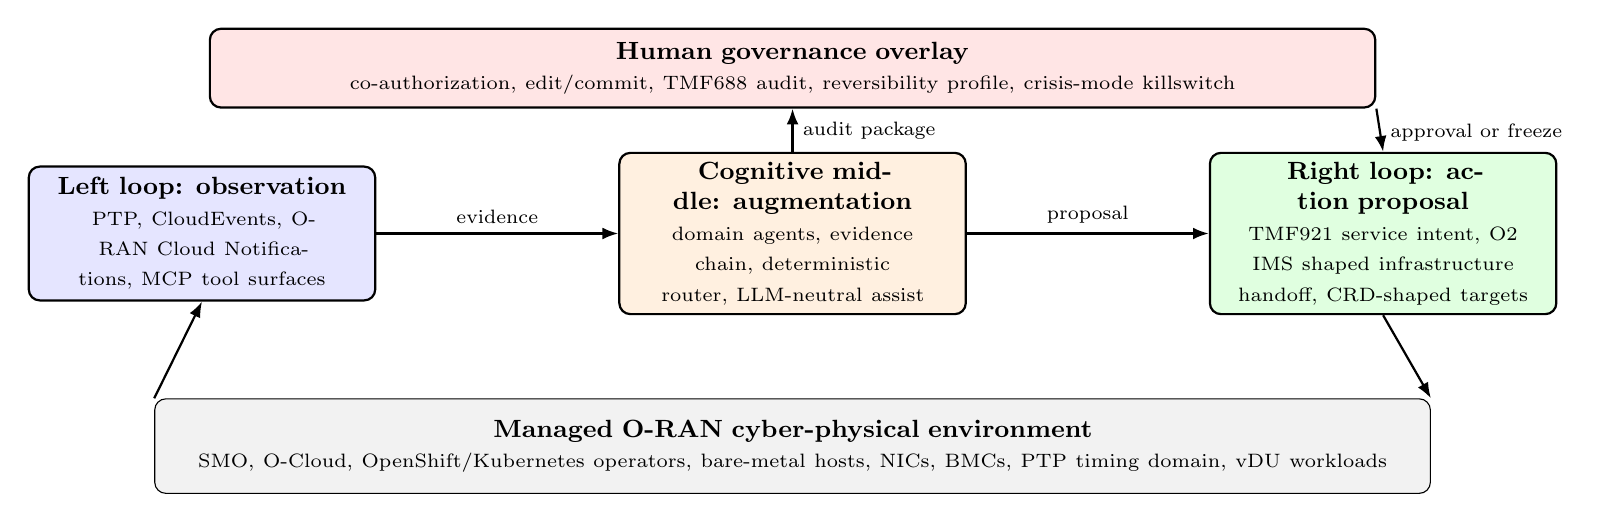
\begin{tikzpicture}[
  env/.style={draw, rounded corners, fill=gray!10, minimum width=16.2cm, text width=15.5cm, minimum height=1.2cm, align=center, font=\small},
  loop/.style={draw, rounded corners, thick, minimum width=4.4cm, text width=4.1cm, minimum height=1.7cm, align=center, font=\small},
  gov/.style={draw, rounded corners, thick, fill=red!10, minimum width=14.8cm, text width=14.0cm, minimum height=1.0cm, align=center, font=\small},
  smallbox/.style={draw, rounded corners, fill=white, minimum width=3.8cm, minimum height=0.42cm, align=center, font=\scriptsize},
  arr/.style={-{Latex[length=2mm]}, thick}
]

\node[env] (environment) at (7.5, -1.1) {\textbf{Managed O-RAN cyber-physical environment}\\\scriptsize SMO, O-Cloud, OpenShift/Kubernetes operators, bare-metal hosts, NICs, BMCs, PTP timing domain, vDU workloads};

\node[loop, fill=blue!10] (left) at (0, 1.6) {\textbf{Left loop: observation}\\\scriptsize PTP, CloudEvents, O-RAN Cloud Notifications, MCP tool surfaces};
\node[loop, fill=orange!12] (middle) at (7.5, 1.6) {\textbf{Cognitive middle: augmentation}\\\scriptsize domain agents, evidence chain, deterministic router, LLM-neutral assist};
\node[loop, fill=green!12] (right) at (15.0, 1.6) {\textbf{Right loop: action proposal}\\\scriptsize TMF921 service intent, O2 IMS shaped infrastructure handoff, CRD-shaped targets};

\node[gov] (governance) at (7.5, 3.7) {\textbf{Human governance overlay}\\\scriptsize co-authorization, edit/commit, TMF688 audit, reversibility profile, crisis-mode killswitch};

\draw[arr] (environment.north west) -- (left.south);
\draw[arr] (left.east) -- node[above, font=\scriptsize] {evidence} (middle.west);
\draw[arr] (middle.east) -- node[above, font=\scriptsize] {proposal} (right.west);
\draw[arr] (right.south) -- (environment.north east);
\draw[arr] (middle.north) -- node[right, font=\scriptsize] {audit package} (governance.south);
\draw[arr] (governance.south east) -- node[pos=0.55, right, font=\scriptsize] {approval or freeze} (right.north);

\end{tikzpicture}}
\caption{Overview architecture. The harness is not the environment and not the operator. It is the cognitive middle that converts observations into bounded, auditable proposals. Human governance spans the point where a proposal may become a physical or service-affecting action.}
\label{fig:overview}
\end{figure*}

\textbf{Left loop: observation.} The left loop converts environmental state into structured evidence. In the timing-domain case, linuxptp and the PTP Operator expose state transitions, cloud-event-proxy emits CloudEvents, and O-RAN Cloud Notifications provide the event payload shape \cite{linuxptp_ptp4l,cloud_event_proxy,cncf_cloudevents,oran_cloud_notifications}. MCP tool surfaces give agents bounded access to platform, RAN, hardware, and O-Cloud facts \cite{mcp_spec,mcp_python_sdk,fastmcp}. The left loop does not decide the remedy; it builds the evidence surface.

\textbf{Cognitive middle: augmentation.} The cognitive middle is the harness. Platform, RAN, and hardware agents converge on an RCA artifact and a candidate \texttt{RemediationProposal}. For covered v0 cases, deterministic routing maps the proposal to service-layer, infrastructure-layer, or ambiguous handling before schema validation and guardrail evaluation. The LLM seam is provider-neutral and non-load-bearing for fixture replay; it can support ambiguous cases through Anthropic, the OpenAI API, or an OpenAI-compatible on-premises vLLM endpoint \cite{litellm}. The critical point is that AI assists the evidence-to-proposal conversion; it does not receive unilateral authority to modify the plant.

\textbf{Right loop: action proposal.} The right loop translates a validated proposal into the proper standards-shaped action surface. Service-layer effects route upward through a TMF921-shaped companion intent \cite{tmf921}. Infrastructure-layer effects route downward through an O2 IMS-shaped dispatch payload toward O-Cloud and Kubernetes-native operator contracts \cite{oran_o2_ims,openshift_mco,kmm_operator,metal3_bmo}. A dual-route case, such as NIC firmware remediation that requires a maintenance window, can produce both an infrastructure handoff and a service coordination intent. In v0, these are dispatch-shape and proposal-shape artifacts, not claims of live production interoperability.

\textbf{Governance overlay.} The governance overlay is not an afterthought. The TMF688-shaped audit event records the evidence, RCA, \texttt{RemediationProposal}, schema result, sandbox verdict, five-subcheck policy guardrail result, companion intent, O2 IMS-shaped dispatch payload, and reversibility profile \cite{tmf688}. The human operator reviews, challenges, edits, co-authorizes, rejects, or freezes. Crisis mode revokes write authority globally. This deliberately slows the last mile of remediation because the last mile can alter physical infrastructure or service availability.

\section{The Intelligence-Augmentation Contract}
\label{sec:contract}

The harness should be evaluated by the quality of the human-machine contract it creates. Table~\ref{tab:contract} summarizes the division of labor.

\begin{table*}[t]
\centering
\small
\begin{tabularx}{\textwidth}{p{3.5cm}X X}
\toprule
Function & Machine responsibility & Human responsibility \\
\midrule
Observation & Collect timing, platform, RAN, hardware, and O-Cloud facts through bounded interfaces. & Decide which operational context matters and whether the incoming fault is inside an approved automation scope. \\
Diagnosis & Produce an RCA artifact with evidence chain and contributing signals. & Challenge weak evidence, add field knowledge, and reject unsupported root-cause claims. \\
Routing & Classify the proposal as service-layer, infrastructure-layer, or ambiguous using deterministic rules first. & Confirm the layer boundary and resolve organizational ownership disputes. \\
Validation & Run sandbox, guardrail, blast-radius, and reversibility checks against committed contracts. & Decide whether the validation is sufficient for the live site and whether additional safeguards are required. \\
Authorization & Assemble a TMF688-shaped audit event and a rollback-aware proposal package. & Edit, approve, defer, reject, or activate the crisis-mode killswitch. \\
Execution & Invoke the gated service or infrastructure handoff only after authorization. & Retain authority for physical change and post-action accountability. \\
\bottomrule
\end{tabularx}
\caption{The intelligence-augmentation contract. The machine compresses evidence, proposal, and validation work. The human retains authority for operational context, exception handling, and physical change.}
\label{tab:contract}
\end{table*}

This contract resolves the most important category error in closed-loop AI operations. The harness can make the operator faster and better informed, but it cannot make the operator unnecessary. In Cloud RAN, a host reboot, NIC firmware update, driver swap, or PTP service change can affect cells, slices, timing, neighboring capacity, and maintenance windows. Those effects cross technical, organizational, and safety boundaries. The operator is therefore not a UI decoration. The operator is the authorization boundary.

The v0 lab makes this contract visible through \texttt{oh-my-tiny-oran} and the read-only \texttt{oran-discover} bundle. The bundle is best understood as six discovery probes plus one pre-flight orchestrator: \texttt{/oran-discover:ptp}, \texttt{/oran-discover:metal3}, \texttt{/oran-discover:redfish}, \texttt{/oran-discover:smo}, \texttt{/oran-discover:taxonomy}, \texttt{/oran-discover:guardrail}, and \texttt{/oran-discover:plan}. It is not an action surface. It is the read-before-write layer that lets the human inspect timing, infrastructure, BMC, SMO intent, taxonomy, and policy state before deciding whether any remediation path deserves authorization.

The Mac-local dashboard exposes the same contract as a reviewer-operable two-loop demo slice of the three-loop architecture: the left loop makes alert and evidence inspection visible, the right loop attaches remediation evidence through a harness-walker \texttt{AuditEvent}, and the cognitive middle remains an augmentation layer rather than an execution authority.

\section{Relationship to the Five-Paper Series}
\label{sec:relationship}

This overview paper is the entry point for a five-paper set. The papers share one remediation spine: observation, RCA, \texttt{RemediationProposal}, schema validation, sandbox and five-subcheck policy guardrail review, human challenge and co-authorization, TMF688-shaped audit, O2 IMS/TMF921 standards-shaped dispatch, and native reconciler execution.

\begin{table*}[t]
\centering
\small
\begin{tabularx}{\textwidth}{p{1.4cm}X X X}
\toprule
Paper & Unique claim & Proof artifact & Out-of-scope \\
\midrule
Paper 0 & Human-governed intelligence augmentation is the correct control frame for closed-loop O-RAN Day-2 remediation. & End-to-end vocabulary tying observation, RCA, proposal, validation, guardrails, audit, dispatch, and reconciler execution into one governance loop. & A new standards interface, autonomous production control, or live O2/SMO interoperability. \\
Paper 1 & The architecture can bridge O2 IMS-shaped infrastructure dispatch to Kubernetes-native operator contracts without giving the agent direct write authority. & O2-IMS-to-operator-CRD bridge pattern, left-loop/cognitive-middle/right-loop decomposition, and CRD-shaped fixtures. & Production O-Cloud Manager deployment, live cluster mutation, or vendor-certified O2 IMS conformance. \\
Paper 2 & The harness composes existing O-RAN, TM Forum, IEEE, DMTF, and Kubernetes-native contracts instead of replacing them. & Standards-lineage bridge map, six v0 bridges, and one prospective R1 seam. & New standards-body proposals, complete coverage of all O-RAN/TMF resources, or normative conformance testing. \\
Paper 3 & Reviewers can falsify the v0 claims through fixture replay and schema-backed verification. & Committed scenarios, citation headers, JSON Schemas, standards-lineage index, and verify gate. & Live production deployment, multi-cluster scale, exhaustive taxonomy coverage, or LLM-dependent proof. \\
Paper 4 & AI nondeterminism can be contained by forcing the cognitive layer to communicate only through deterministic, schema-validated structures. & Structural demarcation model, schema gate, five-subcheck policy guardrail, TMF688/TMF921/O2 IMS-shaped envelopes, and native reconciler delegation. & Raw LLM-generated configuration, direct REST calls to hardware, live Redfish writes, or proof that schemas are standards-body conformance suites. \\
\bottomrule
\end{tabularx}
\caption{Contribution matrix for the five-paper series. Each paper owns a distinct claim, proof artifact, and explicit boundary.}
\label{tab:contribution-matrix}
\end{table*}

The order matters. If a reader starts with the standards-bridge paper, the work can look like a mapping exercise. If a reader starts with the research-harness paper, the work can look like a verification method. If a reader starts with the architecture paper, the work can look like a controller design. If a reader starts with the structural-communication paper, the work can look like an AI safety pattern alone. The overview frame makes clear that the object being designed is a human-governed augmentation loop: observe the environment, produce an RCA, shape a bounded remediation proposal, validate and guardrail it, preserve human challenge and co-authorization, emit standards-shaped audit and dispatch artifacts, and delegate execution to native reconcilers.

\section{Prototype Posture and Limits}
\label{sec:limits}

The v0 repository demonstrates the overview frame in a bounded way. The left loop is represented by committed scenario fault payloads and platform stubs. The cognitive middle contains fixture-covered deterministic routing, schema validation, and guardrail code for covered cases. The right loop contains a Python call into an O2 IMS-shaped stub, committed CRD-shaped fixtures, and TMF921/TMF688-shaped audit and intent envelopes. The verify gate replays five committed scenarios and validates covered v0 claims without a cloud account, live cluster, live SMO, production O2 endpoint, or LLM API key.

Several limits are explicit. The harness does not yet prove live O2 IMS interoperability, live TMF921 interoperability, live Redfish writes, live Kubernetes reconciler commits, or a live R1 exposure. The JSON Schemas are harness-authored research contracts with standards citations, not standards-body conformance suites. The five walkthrough scenarios cover the main delivery branches but not all taxonomy entries. The LLM path is optional support for ambiguous cases; deterministic fixture replay does not depend on any hosted model.

Those limits do not weaken the overview claim. They clarify it. The v0 research artifact demonstrates the proposal shape, dispatch shape, audit shape, guardrail shape, and reversibility-profile shape of human-governed intelligence augmentation. Production interoperability is the v1 work item.

\section{Conclusion}
\label{sec:conclude}

Closed-loop O-RAN Cloud RAN remediation should not be framed as autonomous AI acting on infrastructure. It should be framed as human-governed intelligence augmentation inside a standards-governed cyber-physical operating environment. The shared spine is observation, RCA, \texttt{RemediationProposal}, schema validation, sandbox and five-subcheck policy guardrail review, human challenge and co-authorization, TMF688-shaped audit, O2 IMS/TMF921 standards-shaped dispatch, and native reconciler execution. This overview explains the purpose of the companion architecture, standards-bridge, research-harness, and structural-communication papers: together, they turn that control philosophy into a runnable, bounded, falsifiable, and honestly scoped research artifact.

\section*{Acknowledgements}

This overview builds on a prior multivendor diagnostic substrate co-authored with S. Kiani Mehr, N. Korati Prasanna, M. Vazquez Cebrian, S. Srikanthan, and P. Venkatesh \cite{multivendor_blog_2026}. Source code is Apache-2.0 licensed at \url{https://github.com/dkypuros/oran-agent-harness}.

\bibliographystyle{plain}
\bibliography{refs}

\end{document}
